\section*{Assignment 04: Monetisation Strategy}
\addcontentsline{toc}{section}{Assignment 04: Monetisation Strategy}

In this question I translate our messy spreadsheets into a coherent plan for how SkillSync earns money without suffocating the fragile network effects we are still nurturing.

\subsection*{Revenue streams on the table}
\begin{itemize}
  \item \textbf{Completion fee on each project.} Organisations pay 7\% of the agreed stipend once a project is delivered and rated successful by both sides. It keeps monetisation anchored to the value we already orchestrate, just as \citet{HagiuWright2013} recommend. The fee stays invisible to students so they do not feel priced out.
  \item \textbf{Enablement subscription for organisations.} Larger NGOs and public agencies can upgrade to a "Partner" tier (499 DKK/month) unlocking templated briefs, analytics, and a dedicated coach. This mirrors \citet{Choudary2016}'s argument that platforms should invest in producer tools that raise quality.
  \item \textbf{Talent insights add-on.} Once we accumulate enough data we can sell aggregated skill trend reports to universities and municipal innovation units. We guard against the surveillance trap \citet{Zuboff2019} warns about by applying differential privacy and obtaining explicit consent before monetising any aggregated insights.
  \item \textbf{Grant-backed scholarships.} We plan to pursue social-impact grants that subsidise student stipends for NGOs who cannot afford the completion fee. It is not a profit centre, but it diversifies funding and keeps the marketplace inclusive, aligning with \citet{ShapiroVarian1999}'s note that subsidising one side can accelerate network effects.
\end{itemize}

\subsection*{Timing across the platform lifecycle}
I anchor the roadmap in the classic seed $\rightarrow$ grow $\rightarrow$ harvest logic \citep{Choudary2016}.
\begin{enumerate}
  \item \textbf{Seeding (0--6 months).} No fees, just memoranda of understanding that outline future pricing. We focus on hitting 30 completed projects and building trust rituals (weekly office hours, templated retrospectives).
  \item \textbf{Early growth (months 7--12).} Introduce the 7\% completion fee for new organisations while grandfathering the first cohort for three extra months. Pilot the Partner tier with five agencies that already budget for student collaborations. Success metrics: project completion rate above 85\% and churn below 10\% per quarter.
  \item \textbf{Mature growth (beyond month 12).} Scale the fee to everyone, roll out the Partner tier broadly, and launch the insights add-on for universities. At this stage we track revenue per active organisation, NPS, and uptake of enablement tools to ensure monetisation deepens engagement rather than cannibalising it.
\end{enumerate}

\subsection*{Experiments and guardrails}
To keep ourselves honest we line up three experiments. First, an A/B test on when organisations see the completion fee: at project submission or only after matching. We monitor match acceptance and dropout rates. Second, pricing interviews using the Van Westendorp method to validate the Partner tier before we hard-code the 499 DKK price point; this leans on \citet{Reillier2017}'s advice to co-design producer tools. Third, a diary study with 15 students to learn whether insights reporting feels empowering or creepy, so we can adjust the consent flows. Each experiment has a rollback plan documented in Notion. Writing it out in English keeps the tone scrappy and reflective while answering the exam's monetisation brief directly.

We also mapped the cost side to avoid mistaking top-line revenue for sustainability. Fixed costs in the first year sit around 620,000 DKK (two full-time builders plus design and hosting), while variable costs scale with completed projects (payment processing at 1.4\%, mentor stipends, and customer support hours). Under conservative assumptions we reach operating break-even at roughly 1,050 completed projects per year, a number we can triangulate with the activation roadmap in Assignment~09. The exercise mirrors \citet{ShapiroVarian1999}'s warning that pricing only works if you know your cost curves.

Figure~\ref{fig:student-profile} gives the monetisation story a face. It is the upgraded student profile view that appears when a partner organisation unlocks the enablement subscription. The badges, skill heatmaps, and endorsement timeline are the ``producer tools'' NGOs pay for because they compress due diligence into a glance. Students see immediate value too: the ``next skill to showcase'' recommendation is powered by our data network effect, nudging them towards opportunities that increase platform stickiness. Embedding the screenshot in the paper demonstrates that our monetisation thesis is rooted in actual feature bundles, not abstract spreadsheets.

\begin{figure}[h]
  \centering
  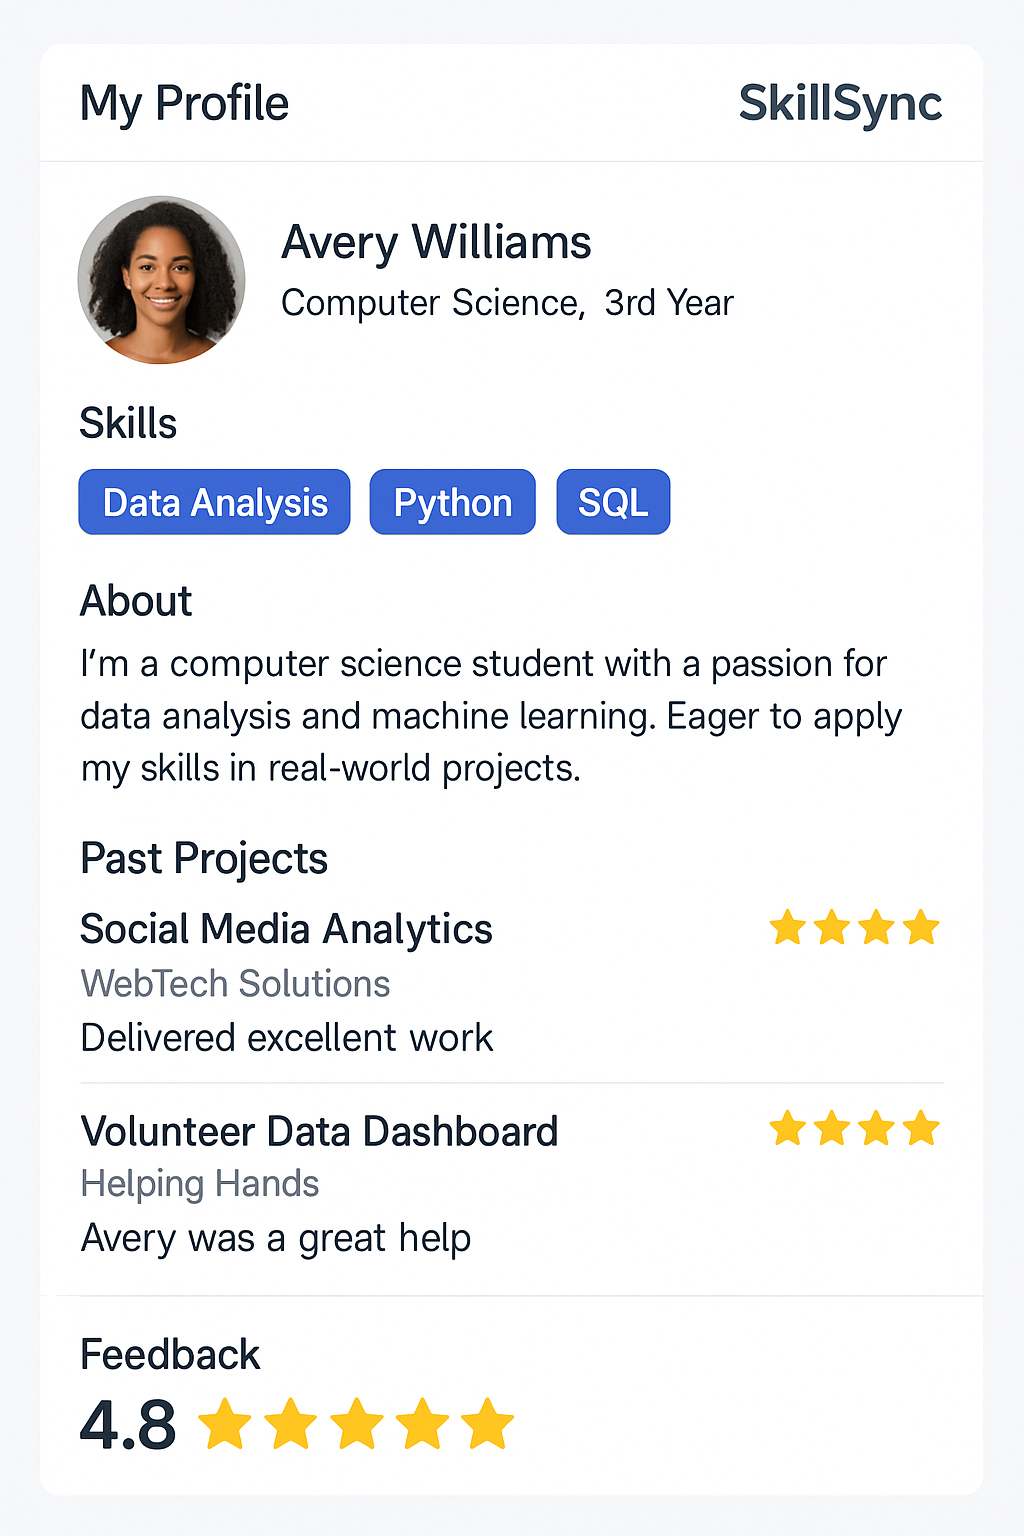
\includegraphics[width=0.8\linewidth]{min-profil-student.png}
  \caption{Enhanced student profile (`min-profil-student.png`) illustrating the Partner enablement features NGOs pay for.}
  \label{fig:student-profile}
\end{figure}

Finally, we pressure-tested ethical boundaries. The talent insights add-on only ships once we have at least five organisations in a sector and 500 completed projects to avoid deanonymisation. Consent flows include explicit ``why we collect this'' copy and easy opt-outs. We also keep grants separate from transaction fees in the ledger so subsidies never distort price signals. Writing these guardrails down honours the spirit of \citet{Zuboff2019} and \citet{Srnicek2017}, who remind platform builders that monetisation can quickly slide into exploitation if data governance lags the business model.
